%!TEX program = xelatex 
% The first line of code is for fontspec package
\documentclass[xcolor={dvipsnames,table}]{beamer}
\let\Tiny=\tiny

\usepackage{amsmath}
\usepackage{graphicx}
\usepackage{booktabs}
\usepackage{tikz} %% design background

%%%%%%%%%%%%%%%%%%%%%%%%%%%%%%%%%%%%%%%%%%%%%%%%%%%%%%%%%%%%%%%%%%%%%%%%%%%%%%%%%%%%
%%%%%%%%%%%%%%%%%%%%% Start Table and Example  %%%%%%%%%%%%%%%%%%%%%%%%%%%%%%%%%%%%%
%%%%%%%%%%%%%%%%%%%%%%%%%%%%%%%%%%%%%%%%%%%%%%%%%%%%%%%%%%%%%%%%%%%%%%%%%%%%%%%%%%%%
\usepackage{makecell, multirow} %% Table
\renewcommand\theadfont{\arraycolor{White}\bfseries}
\newcommand*{\arraycolor}[1]{\protect\leavevmode\color{#1}}
\newcolumntype{A}{>{\columncolor{red!20}}c}
\newcolumntype{B}{>{\columncolor{blue!20}}c}
% Example Colorful Tabular
% \begin{frame}
%     \sffamily
%     \arrayrulecolor{white}
%     \arrayrulewidth=1pt
%     \renewcommand{\arraystretch}{1}
%     \rowcolors[\hline]{2}{.!50!White}{}
%     \resizebox{\linewidth}{!}{%
%         \begin{tabular}{A|A|A|A|A|B|B|B|A}
%             \rowcolor{.!50!Black} % xcolor specification, !<value> represent the shade of a particular color blue!50
%             \multicolumn{5}{A|}{\arraycolor{White}\bfseries 14 subjects} &
%             \multicolumn{3}{B|}{\arraycolor{White}\bfseries 10 subjects} & \\
%             \rowcolor{.!50!Black}
%             \multicolumn{3}{A|}{\arraycolor{White} Surface} &
%             \multicolumn{2}{A|}{\arraycolor{White} Follicle} &
%             \multicolumn{3}{B|}{\arraycolor{White} Surface} &
%             \multirow{-2}{*}{\thead{Control}}\\
%             No les & Non-inf & Inf & Non-inf & Inf & Cheek & Fh & Nose & Mock\\
%         \end{tabular}
%     }%
%     % {\arraycolor{White}\bfseries 14 subjects} change the font color to white and bold the text
% \end{frame} 
%%%%%%%%%%%%%%%%%%%%%%%%%%%%%%%%%%%%%%%%%%%%%%%%%%%%%%%%%%%%%%%%%%%%%%%%%%%%%%%%%%%%
%%%%%%%%%%%%%%%%%%%%% End Table and Example  %%%%%%%%%%%%%%%%%%%%%%%%%%%%%%%%%%%%%%%
%%%%%%%%%%%%%%%%%%%%%%%%%%%%%%%%%%%%%%%%%%%%%%%%%%%%%%%%%%%%%%%%%%%%%%%%%%%%%%%%%%%%


% \setbeamertemplate{sidebar canvas right}{
% \vspace*{235pt}\hspace*{-365pt}%
% {
\includegraphics[height=38pt]{Statistics.png}}}
% \pgfdeclareimage[width = 0.20\paperwidth]{big}{Statistics.png}


%\setbeameroption{show notes} % showing notes for each slides you could include note in each slides by \note{}
%\setbeamertemplate{footline}[frame number]
\setbeamertemplate{headline}{}
%%%%%%%%%%%%%%%%%%%%% START metropolis %%%%%%%%%%%%%%%%%%%%%
\usetheme[block=fill]{metropolis} % A theme from github
\setsansfont[BoldFont={Fira Sans}]{Fira Sans Light} % Must install the corresponding font on the local machine
\setmonofont{Fira Mono}
%%%%%%%%%%%%%%%%%%%%% END metropolis %%%%%%%%%%%%%%%%%%%%%


%%%%%%%%%%%%%%%%%%%%% UKY Colour %%%%%%%%%%%%%%%%%%%%%
\definecolor{UKBlue}{RGB}{0,51,160} % UKY graphic standard primary choice
\definecolor{UKDBlue}{RGB}{32,44,95} % UKY graphic standard secondary choice
\definecolor{UKLBlue}{RGB}{24,151,212}
\setbeamercolor{frametitle}{bg=UKDBlue}
%\setbeamercolor{normal text}{fg=UKDBlue}
\setbeamercolor{alerted text}{fg=UKLBlue}
\setbeamercolor{example text}{fg=UKLBlue}
%%%%%%%%%%%%%%%%%%%%% UKY Colour %%%%%%%%%%%%%%%%%%%%%


\beamertemplatenavigationsymbolsempty % to make presentation looks clean

% \pgfdeclareimage[width=\paperwidth]{mybackground}{UK.png}

% \setbeamertemplate{title page}{

%         \begin{picture}(0,0)

%             \put(-30,-163){%
%                 \pgfuseimage{mybackground}
%             }

%             \put(0,-110.7){%
%                 \begin{minipage}[b][45mm][t]{226mm}
%                     \usebeamerfont{title}{\inserttitle\par}
%                 \end{minipage}
%             }

%             \end{picture}

%     }

\usepackage{xmpmulti}
%\usefonttheme[onlymath]{serif} %% math font theme
%\usetheme{Szeged} % theme for handout
\title{Manifold Learning}
\subtitle{Spring 2018 }
\author{Weihang, Xu}
\date{}

\usepackage{animate}


\begin{document}


\begin{frame}
\titlepage
\end{frame}


\section{Motivation}

\begin{frame}
        % \transduration<0-34>{0}
        % \multiinclude[<+->][format=png, graphics={width=\textwidth}]{something}
        \animategraphics[loop,controls,width=\linewidth]{10}{something-}{0}{34}
\end{frame}

\begin{frame}{Swiss Roll Example}
	\begin{columns}
		\begin{column}{0.5\textwidth}
   			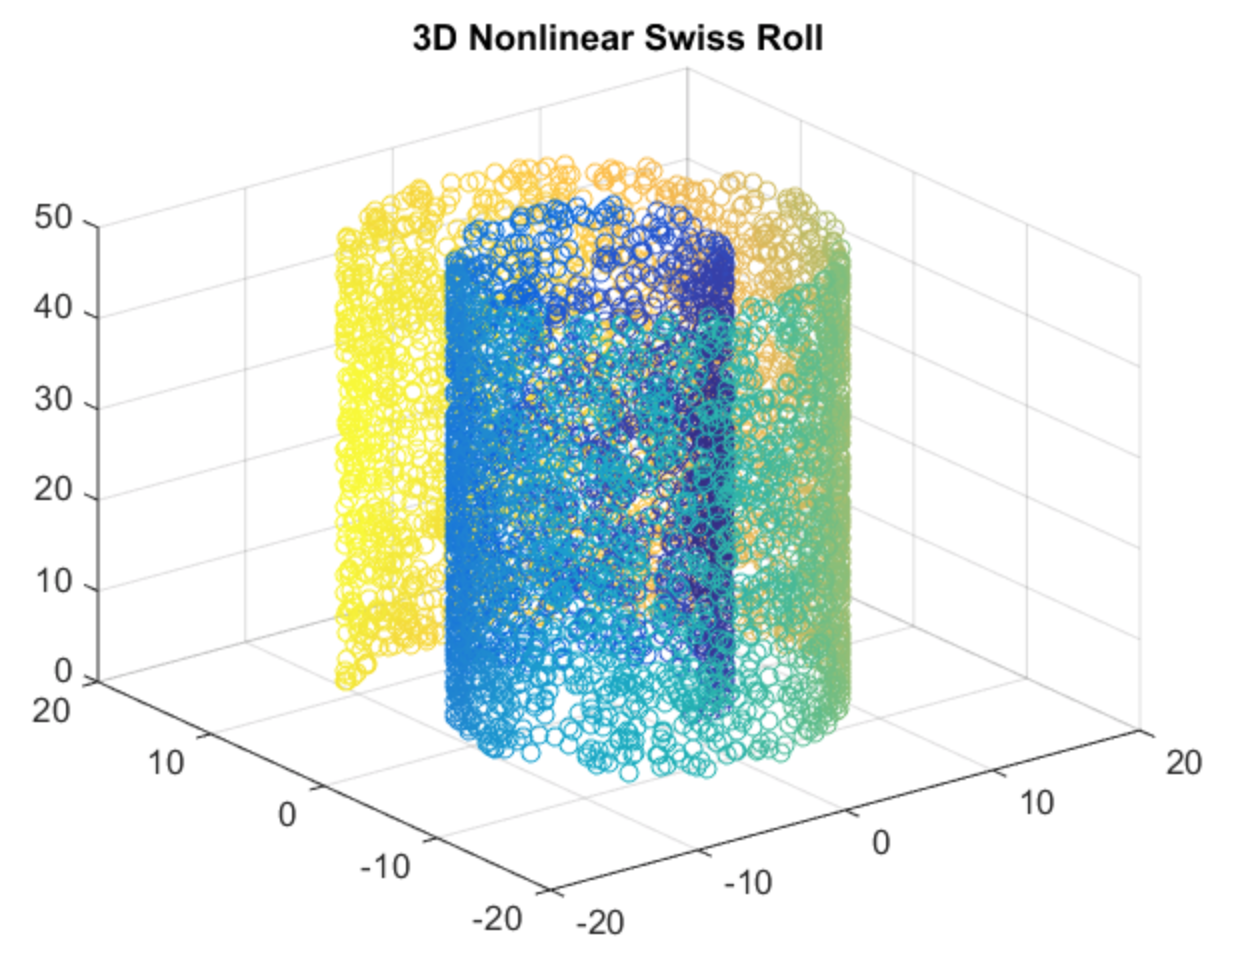
\includegraphics[width=0.9\linewidth]{motive1.png}
		\end{column}
		\begin{column}{0.5\textwidth}  %%<--- here
    		\begin{center}
     		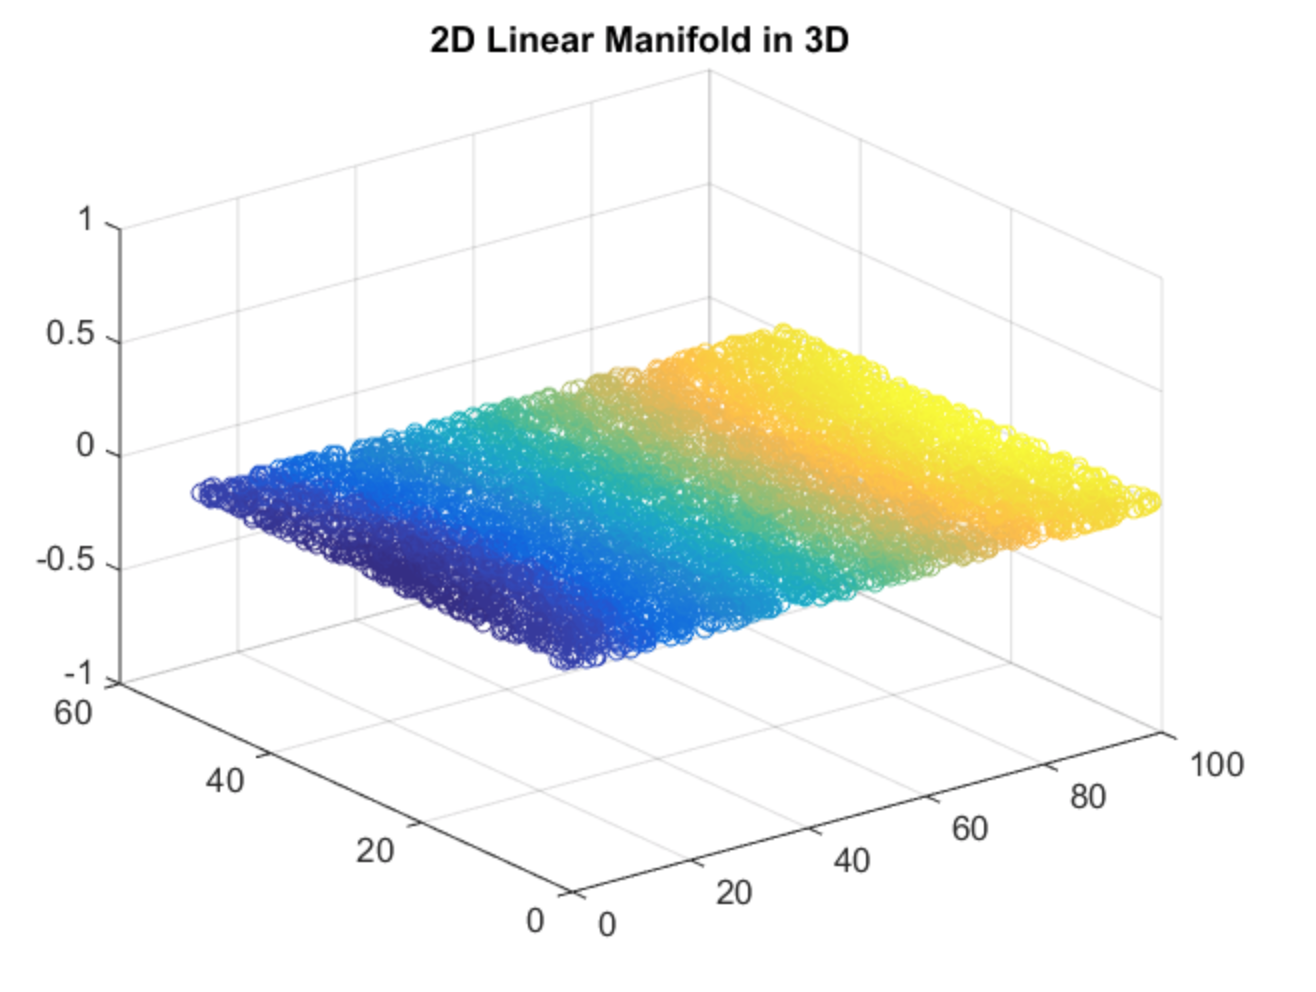
\includegraphics[width=0.9\linewidth]{motive2.png}
     		\end{center}
		\end{column}
	\end{columns}
\end{frame}



\begin{frame}{Swiss Roll Issues}
	\begin{columns}
		\begin{column}{0.5\textwidth}
   			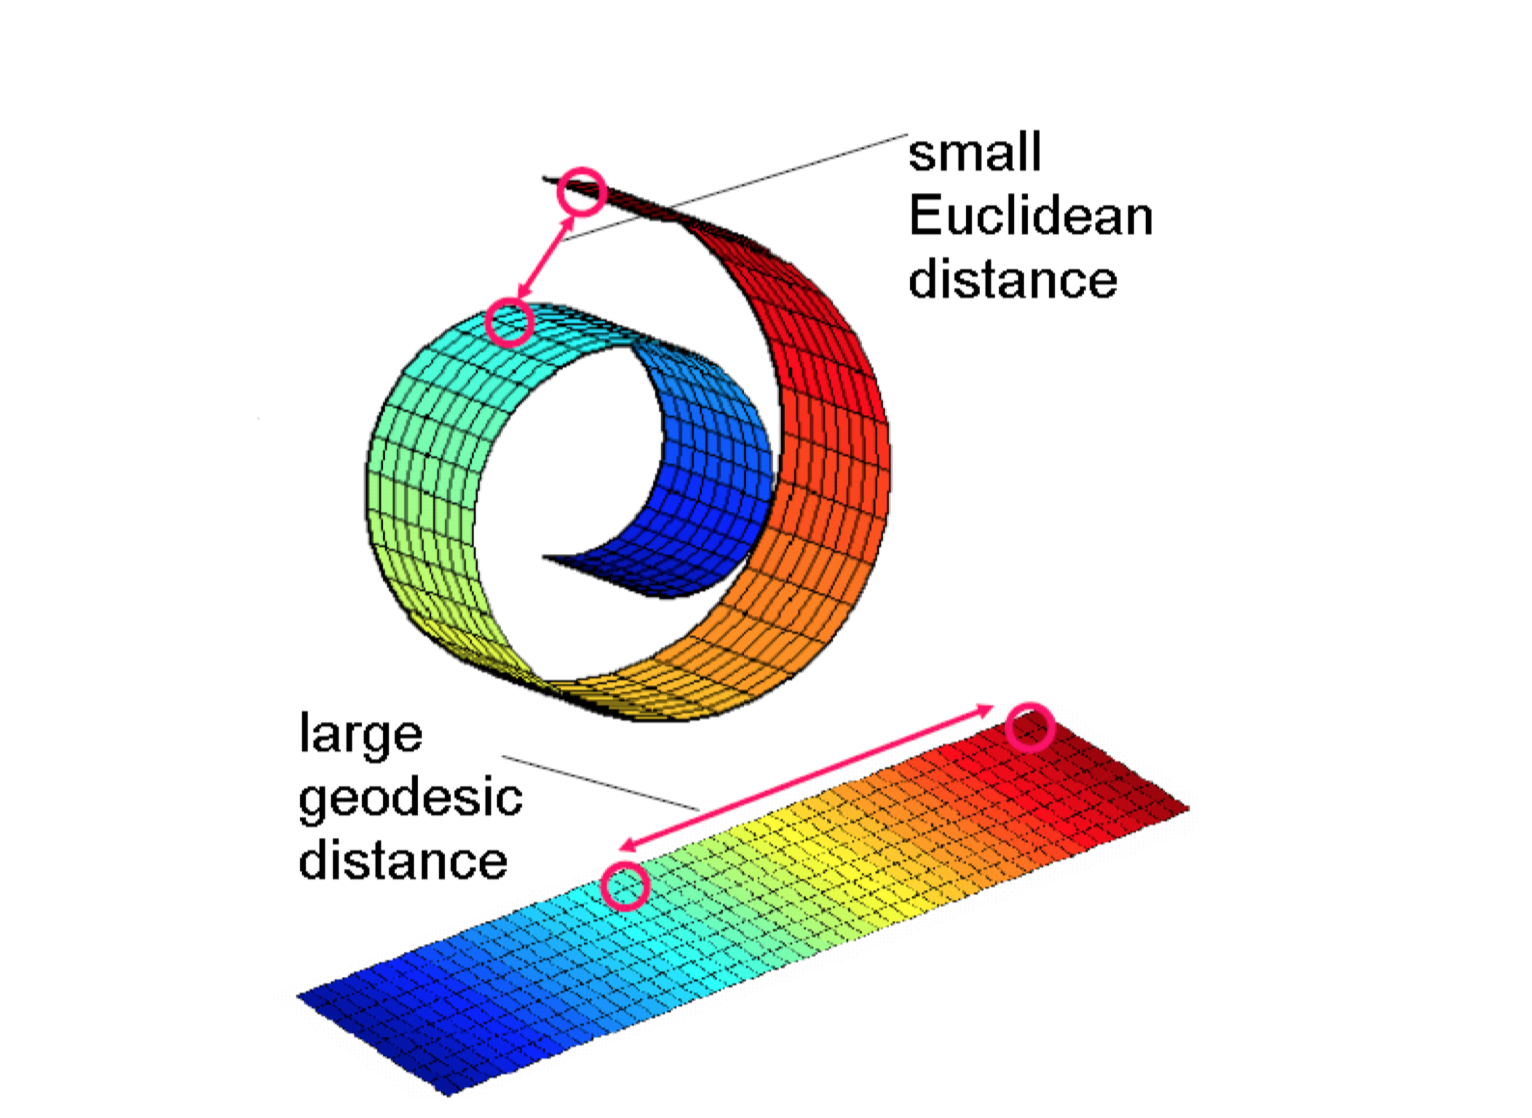
\includegraphics[width=\textwidth]{motive.png}
		\end{column}
		\begin{column}{0.5\textwidth}  %%<--- here
    		\begin{itemize}
     		\item Consider finding clusters in this example.
     		\item We could categorize data points based on their pairwise distance. 
     		\item However, these measurements in the original domain and may not approximate the geodesic distance on the manifold.
     		\end{itemize}
		\end{column}
	\end{columns}
\end{frame}




\section{Manifold Learning}

\begin{frame}{Manifold}
	% The basic intuition behind information theory is that learning that an unlikely event has occurred is more informative than learning that a likely event has occurred. 
	\begin{definition}{ {\em Manifold in metric space} }
		: A manifold is a metric space $M$ such that if $x \in M$, then there is some neighborhood $U$ of $x$ and some integer $n \geq 0$ such that $U$ is homeomorphic to $\mathbb{R}^n$. 
	\end{definition}
	To speak English
	\begin{itemize}
		\item Manifolds are sets look locally like $\mathbb{R}^n$
		\item For instance, the unit circle in $\mathbb{R}^2$ is a manifold with dimension one.
		\item Why do we care about manifold?
	\end{itemize}
	An interesting case arises when the patterns of predictors lie on or near a low dimensional submanifold of the predictor space. In this case, the structure of the data set may be highly nonlinear, and linear methods are bound to fail.
\end{frame}


\begin{frame}{Manifold Learning}
	% The basic intuition behind information theory is that learning that an unlikely event has occurred is more informative than learning that a likely event has occurred. 
	\begin{itemize}
		\item Many real-world data sets are generated with very few degrees of freedom;
		\item An example is pictures of the same object under different imaging conditions, such as rotation angle or translation.
	\end{itemize}
	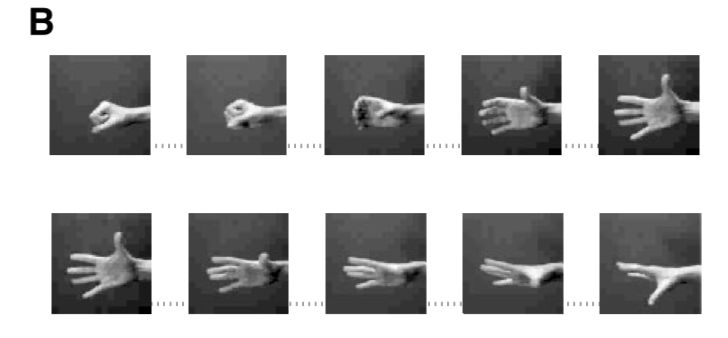
\includegraphics[width=\textwidth]{hand.png}
\end{frame}


\begin{frame}{Manifold Learning}
	% The basic intuition behind information theory is that learning that an unlikely event has occurred is more informative than learning that a likely event has occurred. 
	\begin{itemize}
		\item When these factors vary smoothly, the data points can be seen as lying on a low-dimensional submanifold embedded in the high dimensional ambient space.
		\item Discovering such submanifolds and finding low-dimensional representations of them has been a focus of much recent work on unsupervised learning 
		\item A key theme of these learning algorithms is to preserve (local) topological and geometrical properties (for example, geodesics, proximity, symmetry, angle) while projecting data points to low dimensional representations.
	\end{itemize}
	
\end{frame}

\begin{frame}{Example}
	\begin{center}
     	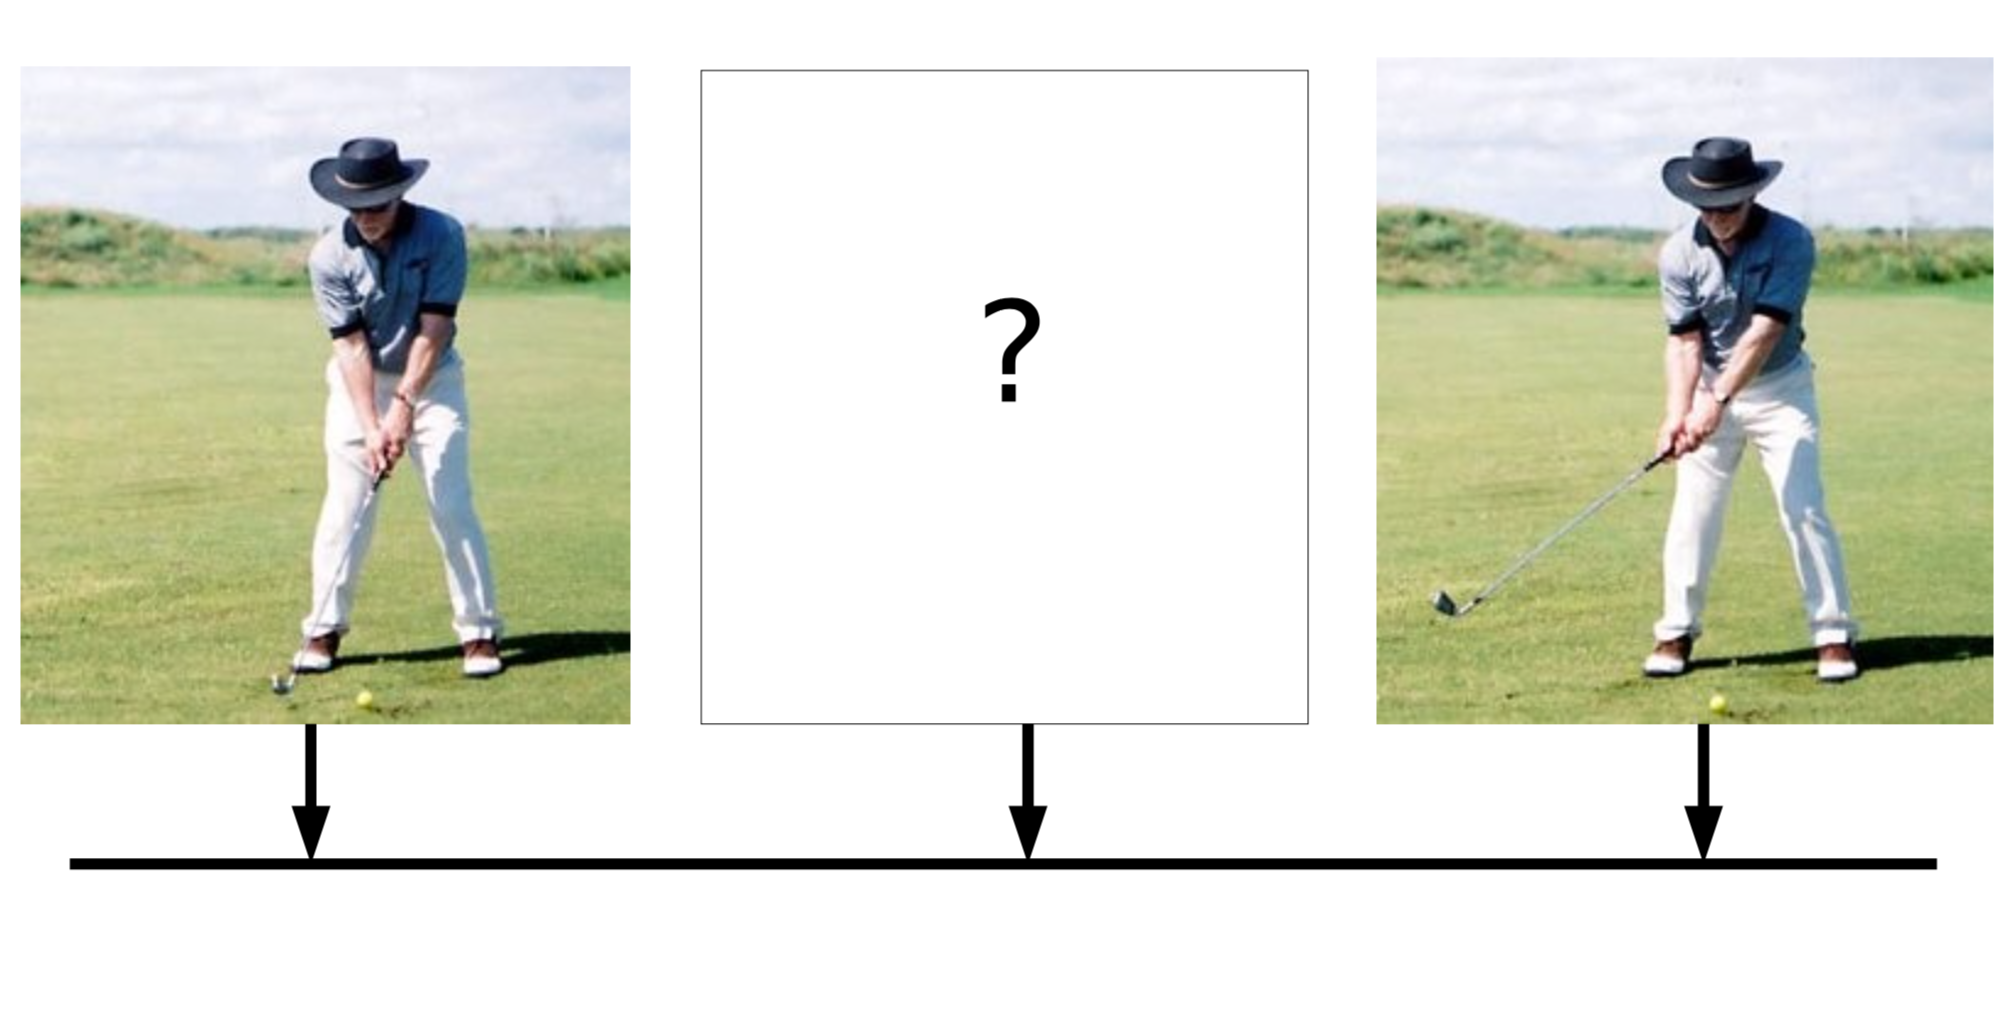
\includegraphics[width=\linewidth]{golf.png}
     \end{center}
\end{frame}

\begin{frame}{Example}
	\begin{center}
     	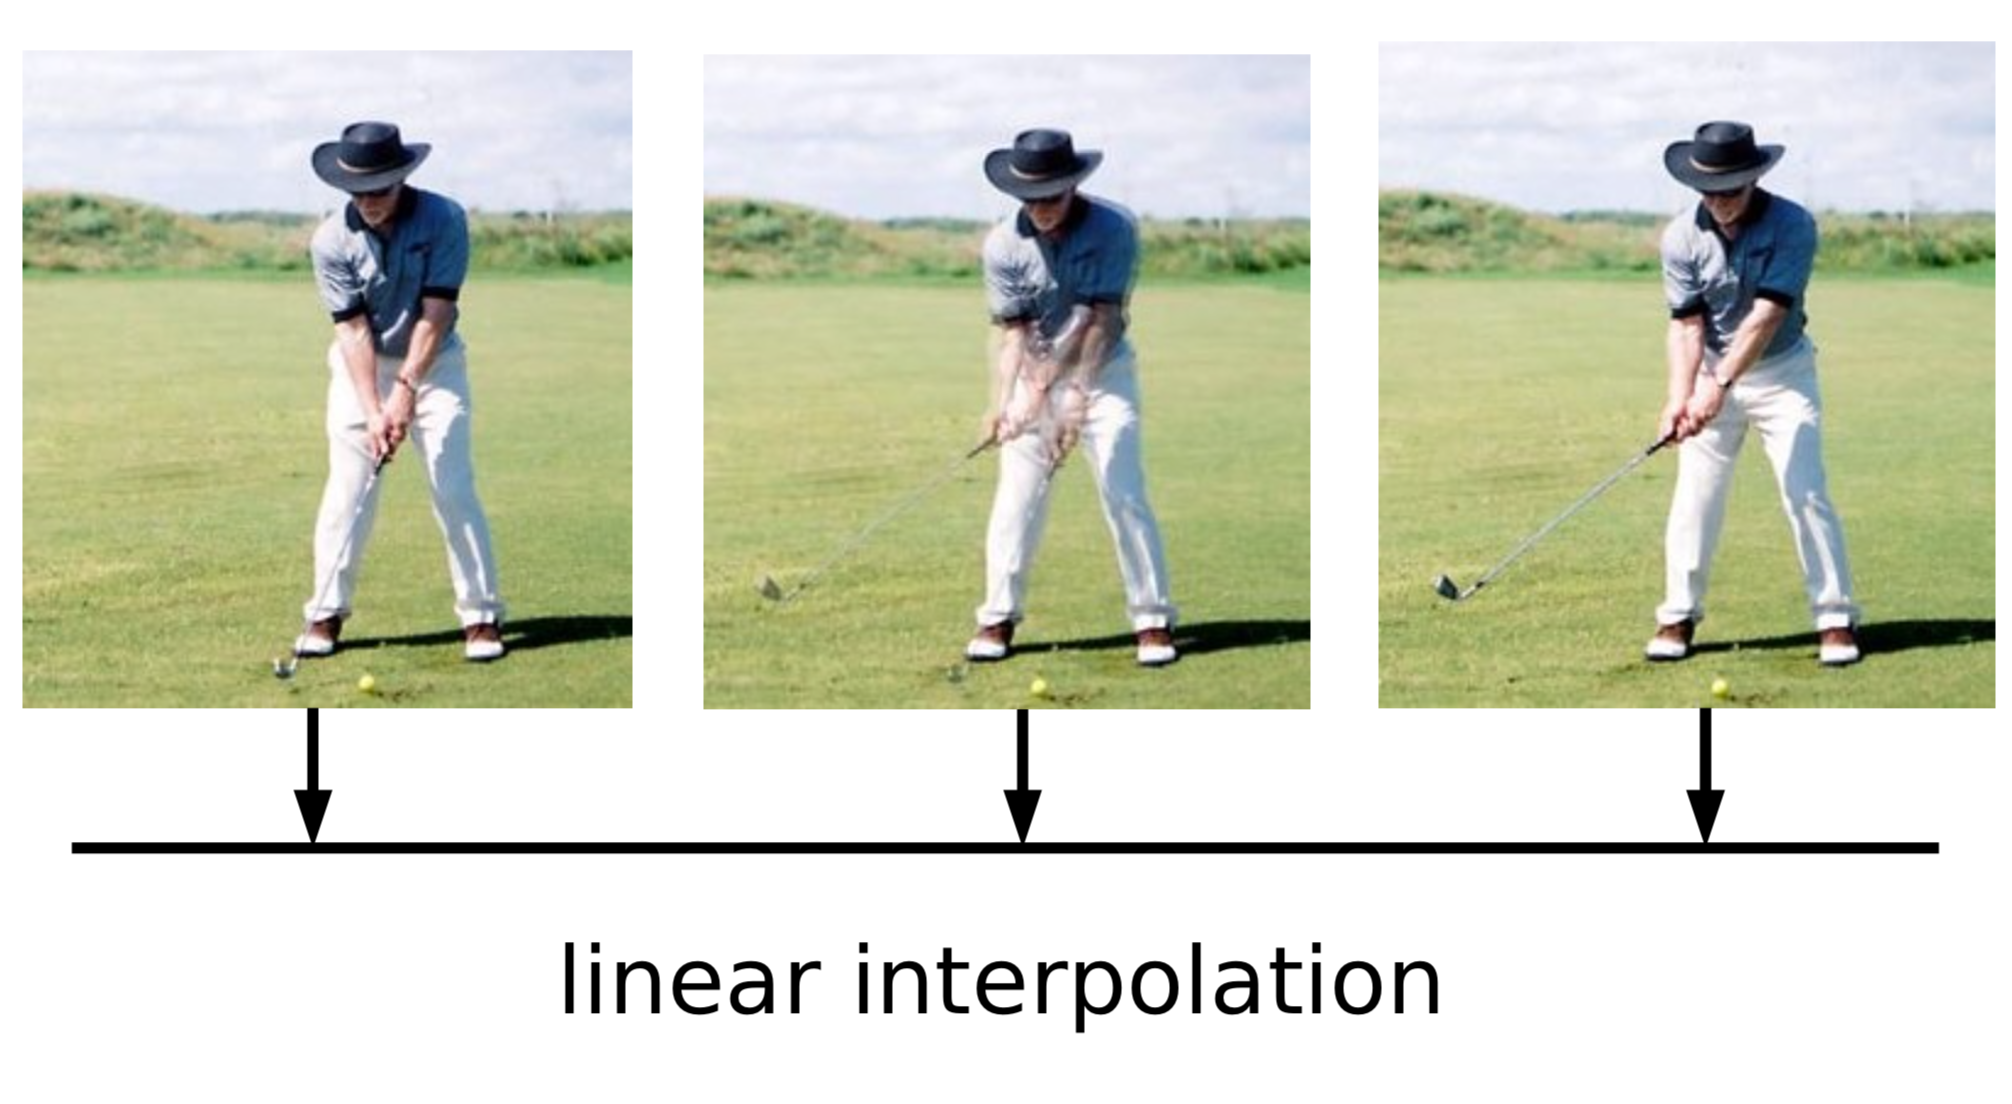
\includegraphics[width=\linewidth]{golfl.png}
     \end{center}
\end{frame}

\begin{frame}{Example}
	\begin{center}
     	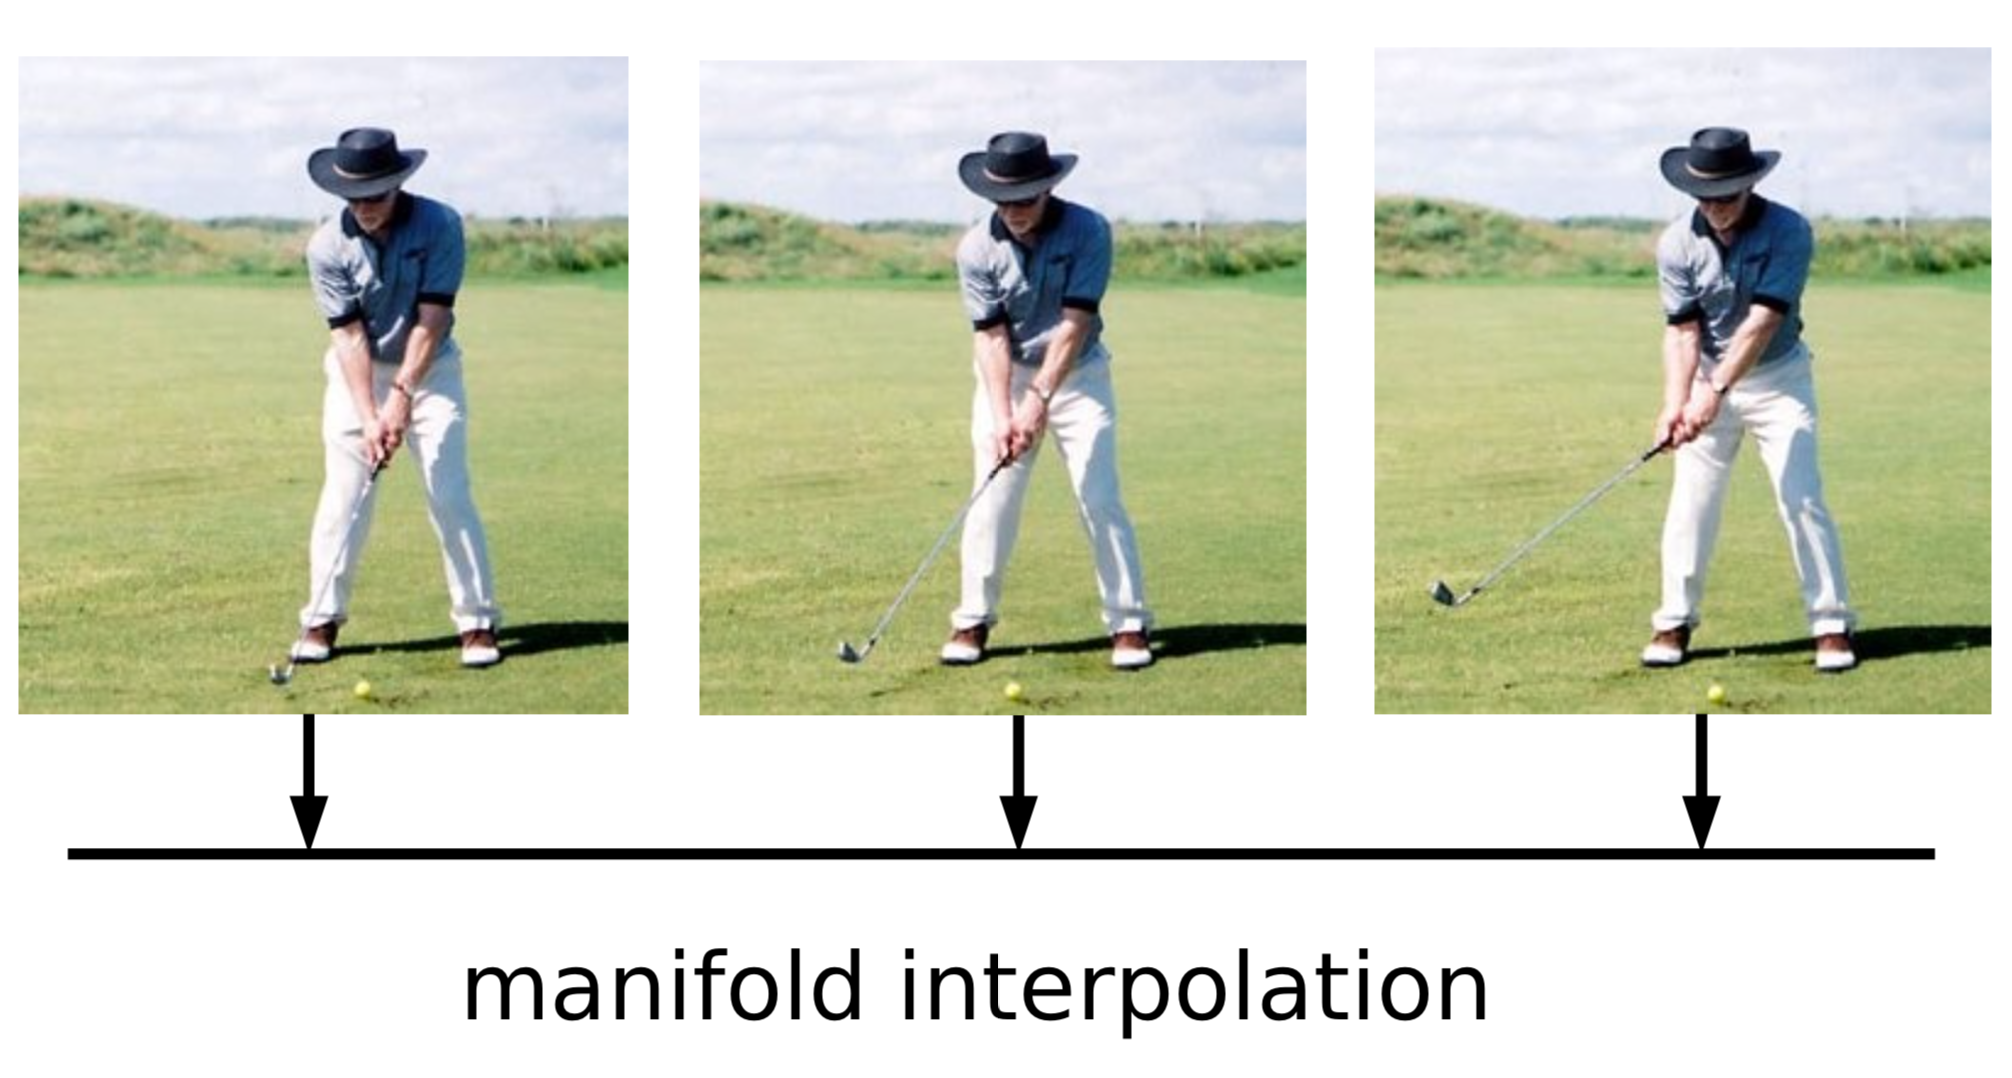
\includegraphics[width=\linewidth]{golfm.png}
     \end{center}
\end{frame}

\section{Isomap}
\begin{frame}{Isomap}
	We want to approximate the geodesic distance on the manifold. Consider this problem with an undirected graph:
	\begin{itemize}
	 	\item Each vertex represent a data point
	 	\item Each edge corresponds to the pairwise distance of the two vertices.
	 \end{itemize}
	\begin{figure}
    \begin{minipage}{0.499\linewidth}{
            \centering
                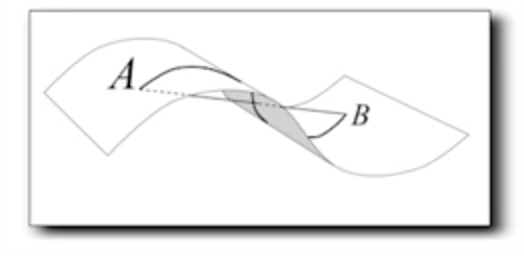
\includegraphics[width=\linewidth]{isoexplain0.png}%            
        }
    \end{minipage}%
    \begin{minipage}{0.499\linewidth}{
            \centering
            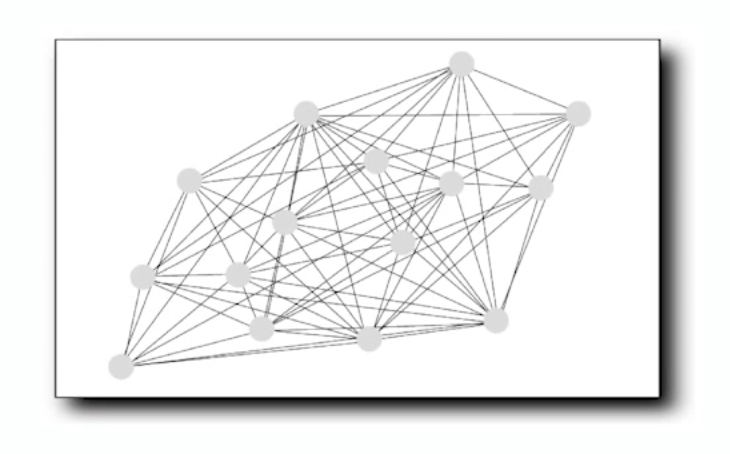
\includegraphics[width=\linewidth]{isoexplain1.png}
        }
    \end{minipage}
\end{figure}
	
\end{frame}

\begin{frame}{Isomap}
	\begin{itemize}
		\item Choose a constraint: A threshold for the distance for each node.
	 	\item Remove edges from the graph, only keep those that satisfy the constraint.
	 	\item Use shortest path in graph to approximate the geodesic distance.
	 \end{itemize}
	\begin{figure}
    \begin{minipage}{0.499\linewidth}{
            \centering
                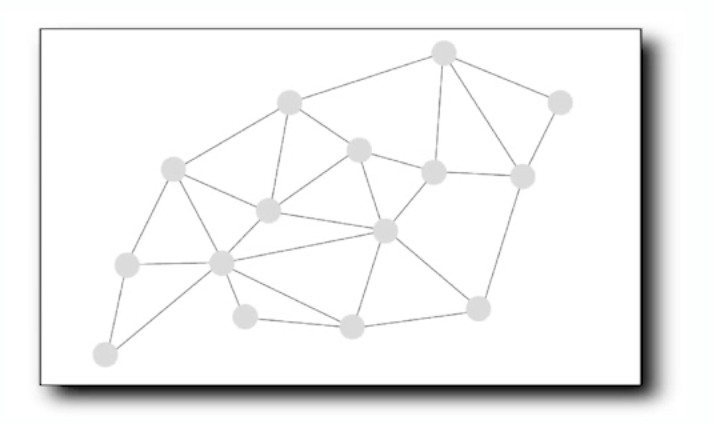
\includegraphics[width=\linewidth]{isoexplain2.png}%            
        }
    \end{minipage}%
    \begin{minipage}{0.499\linewidth}{
            \centering
            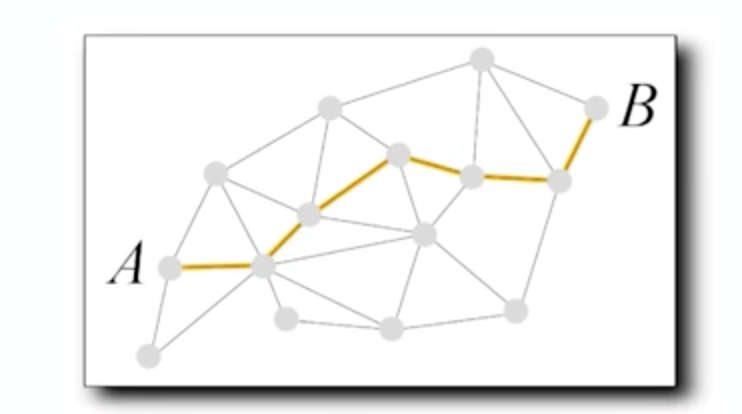
\includegraphics[width=\linewidth]{isoexplain3.png}
        }
    \end{minipage}
\end{figure}
	
\end{frame} 

\begin{frame}{Isomap Algorithm}
	The algorithm has three steps:
	\begin{itemize}
		\item Compute the $k$-nearest neighbors of each input pattern and to construct a graph whose vertices represent input patterns and whose (undirected) edges connect k-nearest neighbors. The edges are then assigned weights based on the Euclidean distance between nearest neighbors.
	 	\item Compute the pairwise distances $d_{ij} = \lVert x_{i} - x_{j}\rVert$ between all nodes $(i,j)$ along shortest paths through the graph. (Djikstra’s algorithm)
	 	\item The pairwise distances $d_{ij}$ from Djikstra’s algorithm are fed as input to MDS, yielding low dimensional outputs $z_{i} \in \mathbb{R}^m$ for which $\lVert z_{i} - z_{j}\rVert \approx d_{ij}$
	 \end{itemize}
\end{frame}


\begin{frame}{Isomap Algorithm}
	\begin{center}
     	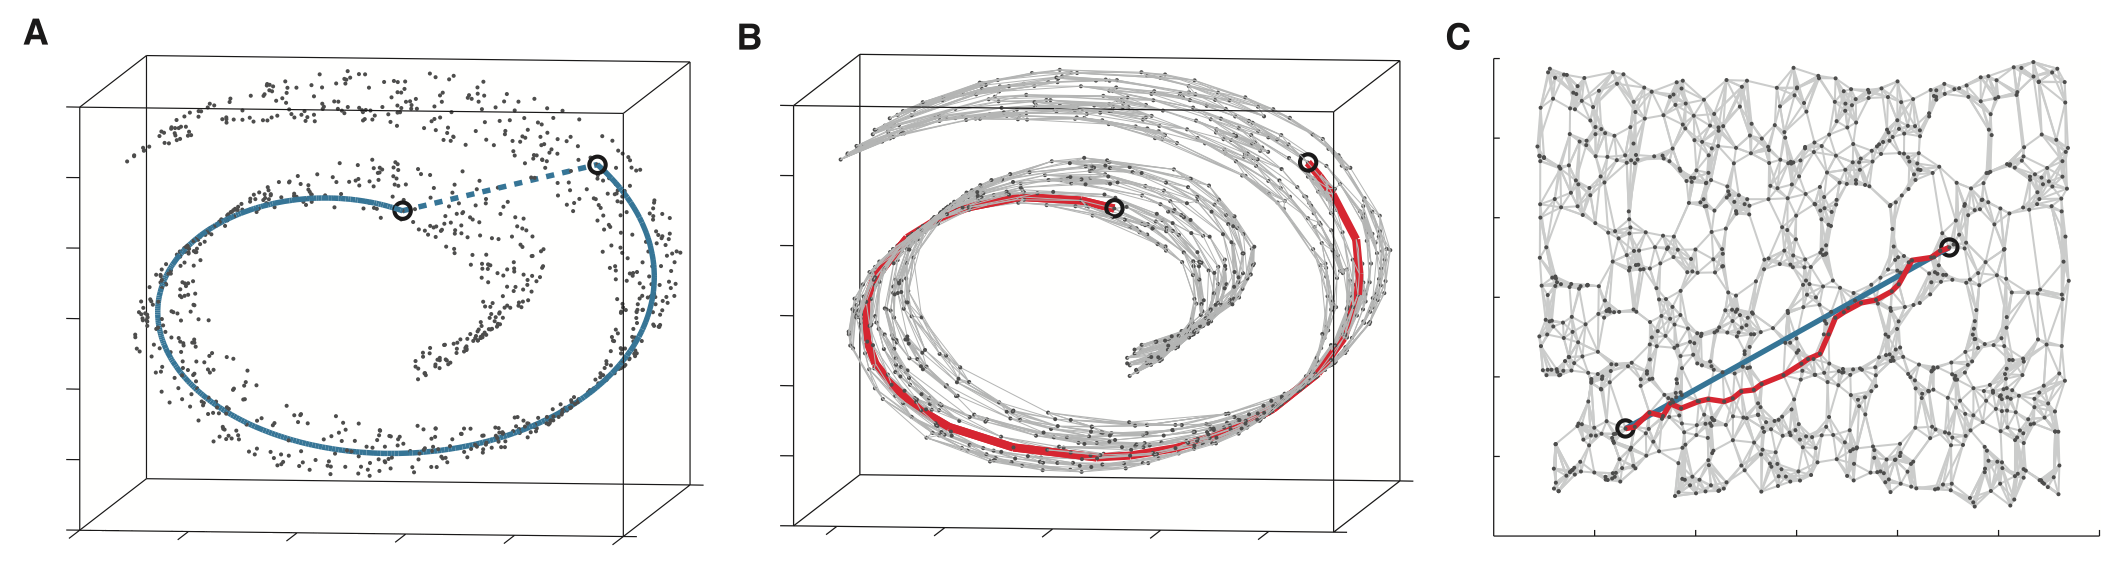
\includegraphics[width=\linewidth]{isosummary.png}
     \end{center}
    When it succeeds, Isomap yields a low dimensional representation in which the Euclidean distances between outputs match the geodesic distances between input patterns on the submanifold from which they were sampled.
\end{frame}

\begin{frame}{Isomap Algorithm}
	\begin{center}
     	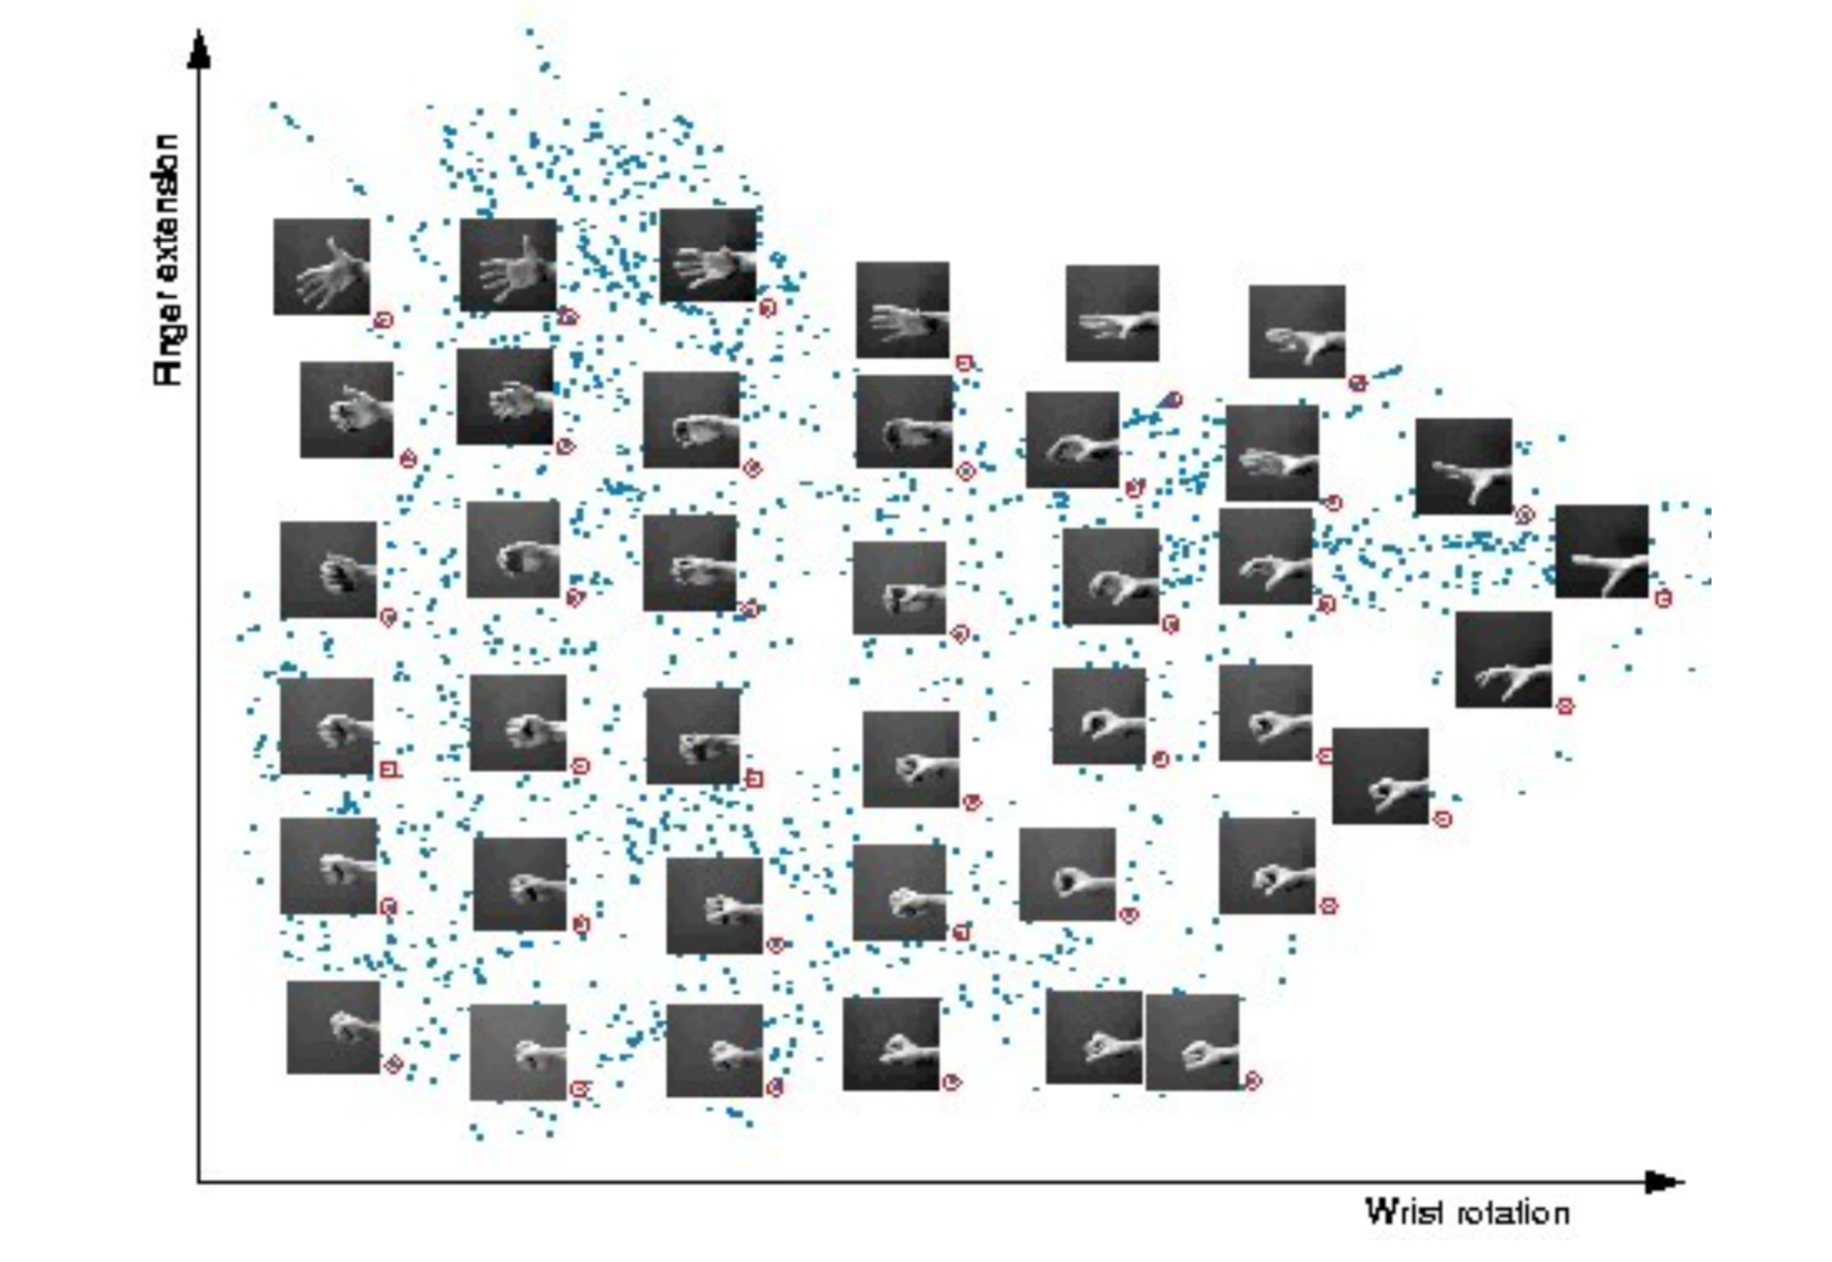
\includegraphics[width=\linewidth]{handresults.png}
     \end{center}
\end{frame}

\begin{frame}{Isomap Pros and Cons}
	\begin{itemize}
		\item preserves global structure
		\item few free parameters
		\item sensitive to noise, noise edges
		\item computationally expensive
	\end{itemize}
\end{frame}



\section{Beyond Isomap}

\begin{frame}{Multidimensional Scaling(MDS)}
Multidimensional scaling seeks values $z_{1},z_{2}, \cdots, z_{n}$ to minimize the so-called {\em stress function}.
$$
S_M(z_{1},z_{2}, \cdots, z_{n}) =\sum_{i \neq j}(d_{ij}-\lVert z_{i} - z_{j}\rVert)^2
$$
This is known as {\em least squares} or {\em Kruskal–Shephard scaling}. The idea is to find a lower-dimensional representation of the data that preserves the pairwise distances as well as possible. Notice that the approximation is in terms of the distances rather than squared distances (which results in slightly messier algebra). A gradient descent algorithm is used to minimize $S_M$.
	
\end{frame}


\begin{frame}{Maximum Variance Unfolding}
	\begin{center}
     	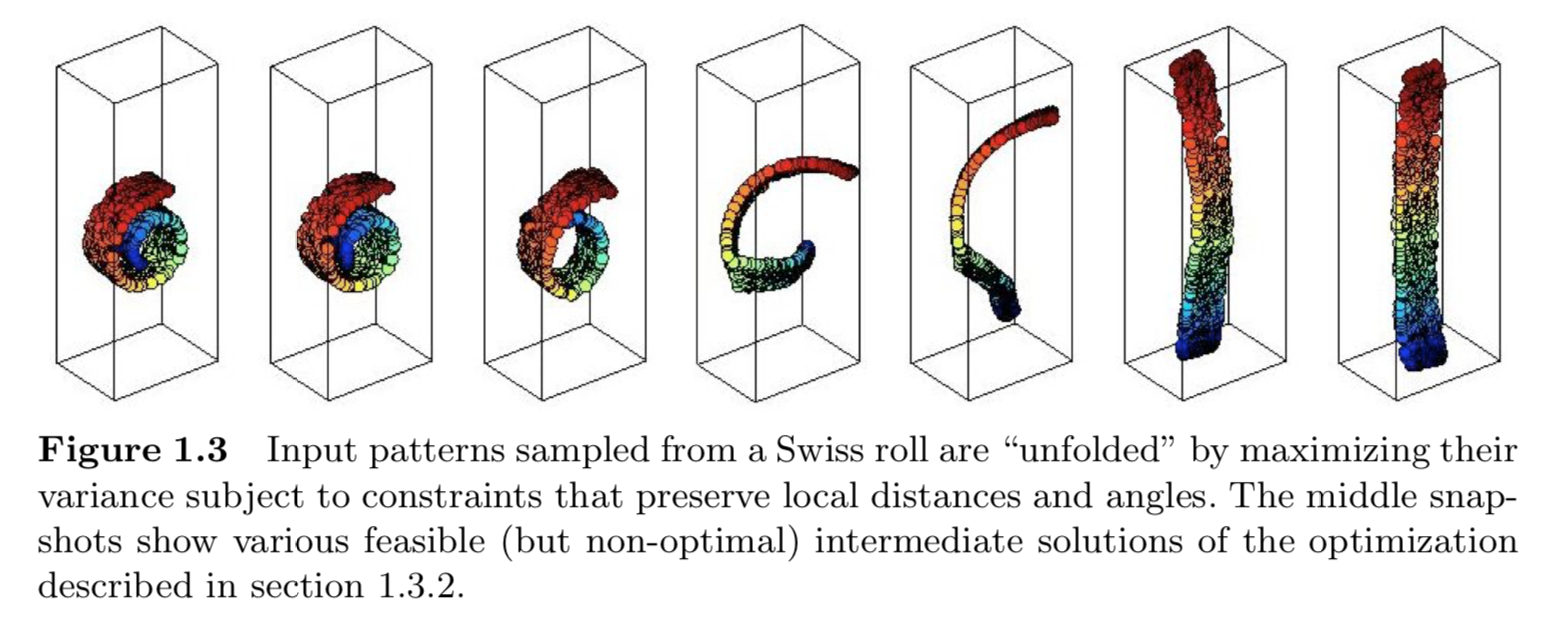
\includegraphics[width=\linewidth]{MVU.png}
     \end{center}
\end{frame}

\section{Reference}


\begin{frame}{Reference}

\begin{thebibliography}{10} 
	\fontsize{1pt}{1}\selectfont 
	 \beamertemplatearticlebibitems
  \bibitem{tenenbaum2000global}
    Tenenbaum, Joshua B and De Silva, Vin and Langford, John C
    \newblock {\em A global geometric framework for nonlinear dimensionality reduction}
    \newblock science 290 5500 2319--2323, 2000. 
  \beamertemplatebookbibitems
  \bibitem{friedman2001elements}
    Friedman, Jerome and Hastie, Trevor and Tibshirani, Robert.
    \newblock {\em The elements of statistical learning}.
    \newblock Springer series in statistics New York, 2001.
  \beamertemplatebookbibitems
  \bibitem{spivak1979comprehensive}
    Spivak, Michael
    \newblock {\em A comprehensive introduction to differential geometry}.
    \newblock Publish or perish, 1979.
  \beamertemplatearticlebibitems
  \bibitem{saul2006spectral}
    Saul, Lawrence K and Weinberger, Kilian Q and Ham, Jihun H and Sha, Fei and Lee, Daniel D
    \newblock {\em Spectral methods for dimensionality reduction}
    \newblock Semisupervised learning, 293--308, 2006.
 
  \beamertemplatearticlebibitems
  \bibitem{nilsson2007regression}
    Nilsson, Jens and Sha, Fei and Jordan, Michael I
    \newblock {\em Regression on manifolds using kernel dimension reduction}
    \newblock Proceedings of the 24th international conference on Machine learning 697--704, 2007.
  \end{thebibliography}

\end{frame}


\end{document}
